\subsection{补充材料：来源索引与全部比较}
\label{sec:supplement}

每个厚度数值都应能沿着波段回到原始光谱。本节先列源附件与行号，再将路线比较、逐块检验和区间计数分开保存，使同一晶圆的角度差异与不同计算条件各有对应的观测对象。

\subsubsection{来源索引：附件行号连接共同波段}

源附件按材料和入射角定位，波段按原工作表行号定位。四个附件共享的坐标共有7469点，表\ref{tab:supp-source}将其归回两块晶圆；图\ref{fig:raw-anomaly}保留原始异常，图\ref{fig:common-coordinate}标出共同拟合区段，光学资料的已知与缺项则对应表\ref{tab:available-info}。
% src:交接/数据档案.json:总览.附件总数;总览.四文件共有波数点数;总览.独立晶圆数
% src:求解/问题1/结果/实测输入核验.json:共同原始波数点数

\begingroup
\small
\begin{longtable}{>{\centering\arraybackslash}p{0.14\textwidth}>{\centering\arraybackslash}p{0.18\textwidth}>{\centering\arraybackslash}p{0.12\textwidth}>{\centering\arraybackslash}p{0.20\textwidth}>{\centering\arraybackslash}p{0.20\textwidth}}
\caption{四个源附件的材料与工作表行号}\label{tab:supp-source}\\
\toprule
源附件 & 材料 & 入射角 & 原始数据行 & 数据列 \\
\midrule
\endfirsthead
\toprule
源附件 & 材料 & 入射角 & 原始数据行 & 数据列 \\
\midrule
\endhead
附件一 & 碳化硅 & $10^\circ$ & 2--7470 & 波数、反射率 \\
附件二 & 碳化硅 & $15^\circ$ & 2--7470 & 波数、反射率 \\
附件三 & 硅 & $10^\circ$ & 2--7470 & 波数、反射率 \\
附件四 & 硅 & $15^\circ$ & 2--7470 & 波数、反射率 \\
\bottomrule
\end{longtable}
\endgroup
% src:交接/数据档案.json:文件档案.0.材料;文件档案.0.入射角度;文件档案.1.材料;文件档案.1.入射角度;文件档案.2.材料;文件档案.2.入射角度;文件档案.3.材料;文件档案.3.入射角度;下游读取规范.数据首行从一计数;下游读取规范.数据末行从一计数

行号包含表头，均指源工作簿的首个工作表；波数列和反射率列分别位于左列与右列。因同材料两角的坐标逐行一致，联合计算直接配对原始行，不先平均反射率，也不通过插值改变观测位置。

主窗口为$1200$--$3800\ \mathrm{cm}^{-1}$，表\ref{tab:supp-window}把参与拟合的波段与原始行号并排定位。
% src:求解/问题2/结果/数据审查.json:主窗口_cm^-1

附件二的超百反射率段为$801.28$--$927.11\ \mathrm{cm}^{-1}$。它与主窗口没有交集，因此主窗口的路线差异并非裁掉异常值所带来的改善。
% src:交接/数据档案.json:文件档案.1.工作表.0.反射率检查.超过百分之百区段.0.起始波数;文件档案.1.工作表.0.反射率检查.超过百分之百区段.0.终止波数

\begingroup
\small
\begin{longtable}{>{\centering\arraybackslash}p{0.20\textwidth}>{\centering\arraybackslash}p{0.29\textwidth}>{\centering\arraybackslash}p{0.19\textwidth}>{\centering\arraybackslash}p{0.20\textwidth}}
\caption{原始波段及参与计算的点数}\label{tab:supp-window}\\
\toprule
对象 & 波数区间（$\mathrm{cm}^{-1}$） & 原始行号 & 每谱点数 \\
\midrule
\endfirsthead
\toprule
对象 & 波数区间（$\mathrm{cm}^{-1}$） & 原始行号 & 每谱点数 \\
\midrule
\endhead
四谱全段 & 399.6747--4000.1220 & 2--7470 & 7469 \\
四谱主窗口 & 1200--3800 & 1663--7054 & 5392 \\
连续留段点集 & 1200.470--3799.562 & 主窗口内选点 & 480 \\
附件二超百段 & 801.2780--927.1104 & 835--1096 & 262 \\
四谱共同首点 & 399.6747 & 2 & 1 \\
\bottomrule
\end{longtable}
\endgroup
% src:求解/问题1/结果/实测输入核验.json:共同原始波数点数;波数范围_每厘米
% src:求解/问题2/结果/数据审查.json:主窗口_cm^-1;共同窗口原始点数_每角度;抽样点数_每角度;抽样索引.0;抽样索引.479
% src:交接/数据档案.json:文件档案.1.工作表.0.反射率检查.超过百分之百区段.0;文件档案.1.工作表.0.反射率检查.零值点.0

\begin{figure}[!htb]
    \centering
    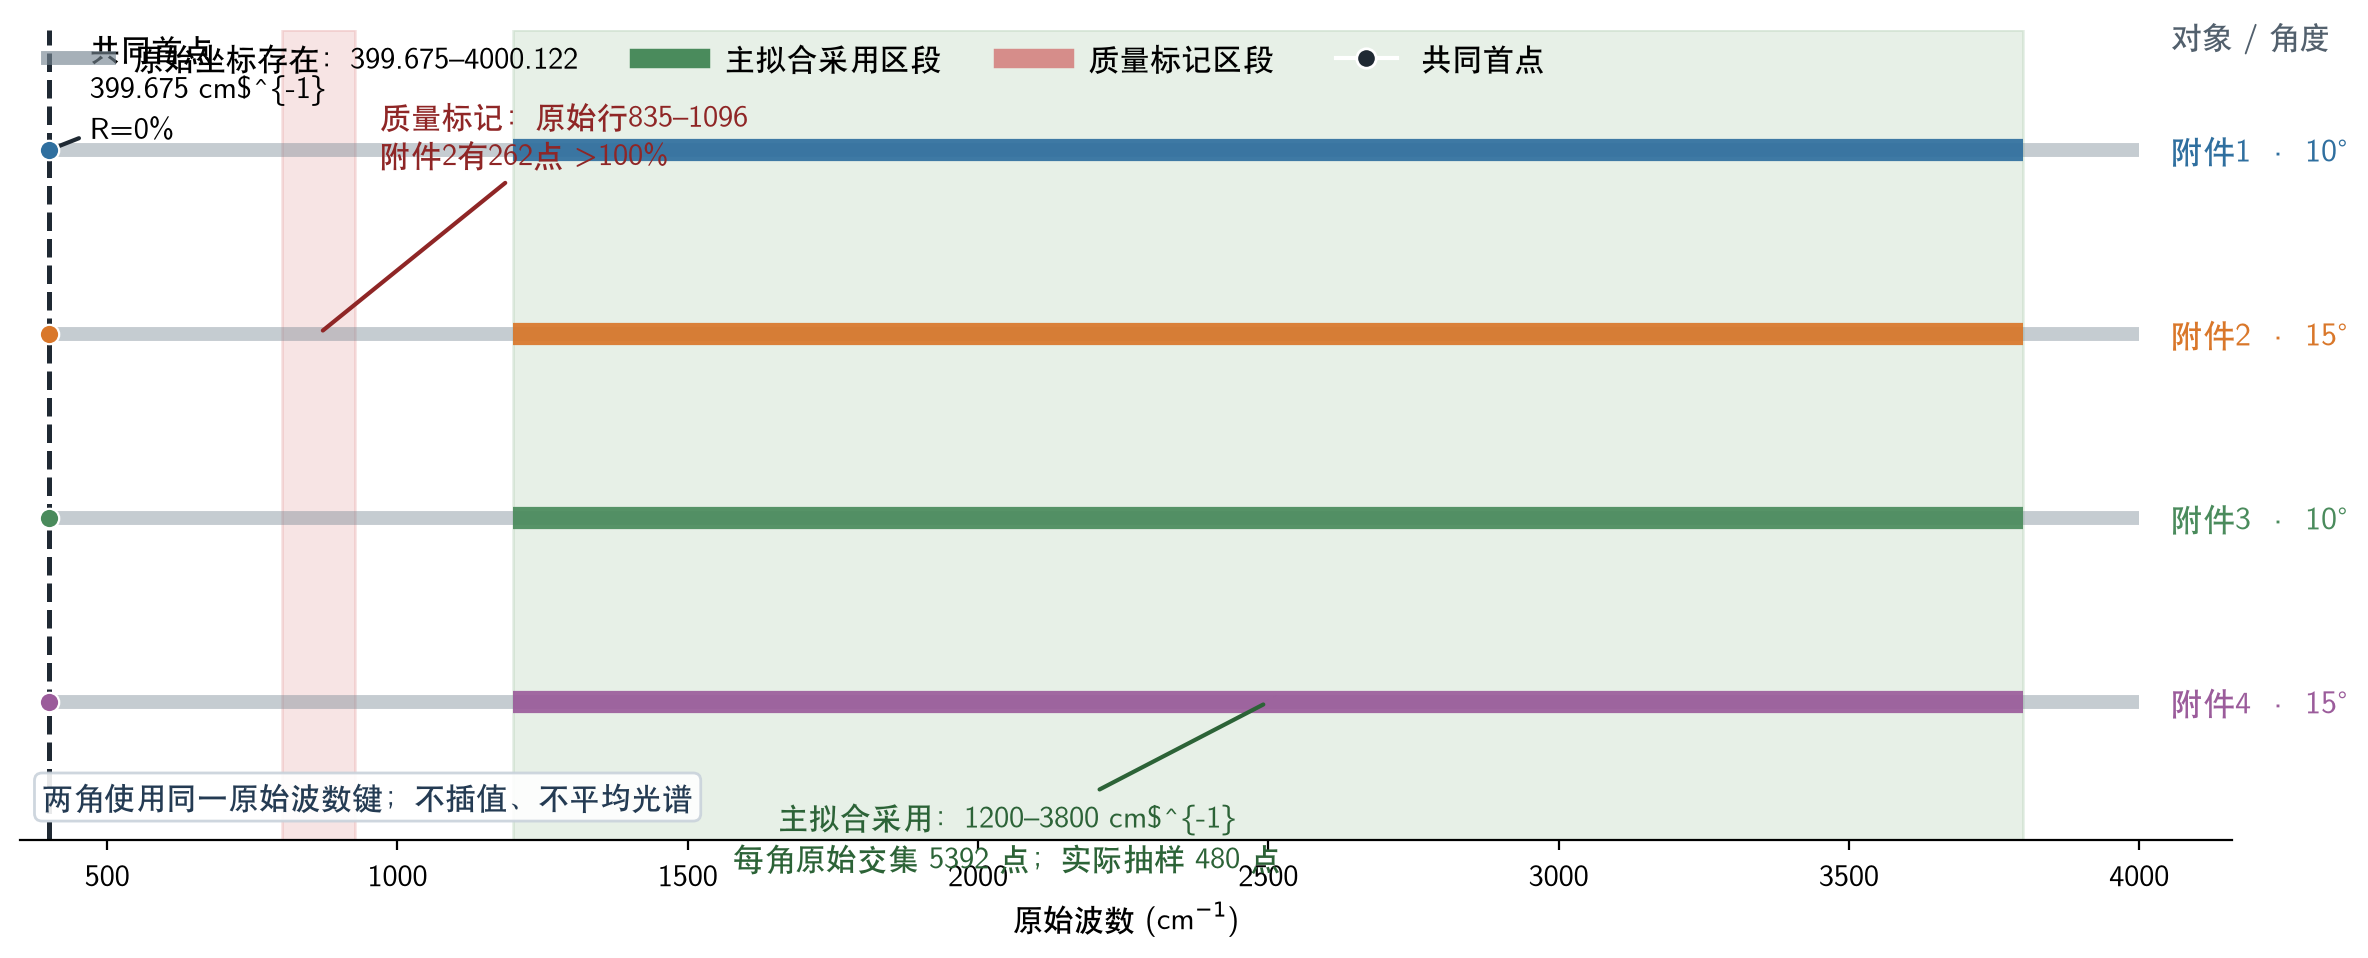
\includegraphics[width=0.8\textwidth]{../求解/公共/图片/共同坐标标记质量区段.png}
    \caption{四谱共同波数坐标及拟合区段}
    \label{fig:common-coordinate}
\end{figure}

抽样点集与全量点集承担不同任务：前者使各路线在同一组连续区段上比较，后者用于硅的主窗口整体拟合。共同抽样的480个点可由式\eqref{eq:supp-source-row}逐点回到工作表行号，而不是只知道所在波段。
% src:求解/问题2/结果/数据审查.json:抽样点数_每角度;抽样索引

\begin{equation}
\ell_j=1663+\left\lfloor\frac{5391j}{479}\right\rfloor,
\qquad j=0,\ldots,479.
\label{eq:supp-source-row}
\end{equation}
% src:求解/问题2/结果/数据审查.json:抽样索引;共同窗口原始点数_每角度;抽样点数_每角度
其中，$j$为从零起算的共同抽样序号，$\ell_j$为包含表头的源工作表行号，$\lfloor\cdot\rfloor$表示向下取整。同一序号在四个附件中对应相同波数，但反射率仍分别取各自原值；原始波段、角度和行号确定后，路线优劣才有共同的比较对象。

\subsubsection{路线比较：合成回收与实测预测分列}

路线比较先区分是否知道真实厚度。早期曾考虑直接用观测光谱衡量测厚误差，但附件缺少厚度真值和折射率曲线，因而改在原始共同坐标上构造24例已知光学条件的合成光谱；这一实际取舍决定了图\ref{fig:08}和表\ref{tab:04}中的误差衡量方法回收能力，而实测留段误差衡量谱形预测。
% src:交接/实验记录.json:22.尝试;22.现象;22.决定
% src:求解/问题1/结果/合成验证.json:分组汇总.共同匹配.案例数

双束界面场反演在原型共同案例上的平均相对误差为$0.0010\%$，正式共同匹配组为$0.0008\%$。表\ref{tab:supp-q1-routes}保留两个阶段的数值而不相互替换；新增匹配与故意改变光学关系的情景也单列，避免把匹配条件下的回收表现说成所有情景下的测厚精度。
% src:求解/问题1/原型结果/路线2.json:核心指标.合成厚度平均相对误差_百分比
% src:求解/问题1/结果/合成验证.json:主指标.数值

\begingroup
\small
\begin{longtable}{>{\centering\arraybackslash}p{0.18\textwidth}>{\centering\arraybackslash}p{0.30\textwidth}>{\centering\arraybackslash}p{0.14\textwidth}>{\centering\arraybackslash}p{0.26\textwidth}}
\caption{问题一原型与正式合成误差}\label{tab:supp-q1-routes}\\
\toprule
数据阶段 & 方法或情景 & 案例数 & 平均误差（\%） \\
\midrule
\endfirsthead
\toprule
数据阶段 & 方法或情景 & 案例数 & 平均误差（\%） \\
\midrule
\endhead
原型合成 & 色散峰序反演 & 24 & 0.0201 \\
原型合成 & 双束界面场反演 & 24 & 0.0010 \\
原型合成 & 连续相位拟厚 & 24 & 0.0041 \\
正式合成 & 共同匹配 & 24 & 0.0008 \\
正式合成 & 新增匹配 & 16 & 0.0011 \\
正式合成 & 模型失配 & 10 & 0.3028 \\
正式合成 & 常折射率峰距 & 24 & 2.5875 \\
\bottomrule
\end{longtable}
\endgroup
% src:求解/问题1/原型结果/路线1.json:主指标值;参数情景.组合数
% src:求解/问题1/原型结果/路线2.json:核心指标.合成厚度平均相对误差_百分比
% src:求解/问题1/原型结果/路线3.json:主指标值
% src:求解/问题1/结果/合成验证.json:分组汇总;常折射率峰距基线

模型失配组改变的是生成观测的光学关系，而非删除困难案例后重新计分；因此它回答的是模型假设改变时的误差增长。原型与正式共同组虽然同属已知光学条件比较，含噪观测和估计步骤均有所不同，应按阶段各自对照。

碳化硅正式留段误差为$1.2074$，二次趋势对照为$1.4404$，均为无量纲谱形误差。这里的标准化误差，是每块反射率误差除以该折该角训练残差的四分位距，再对测试块等权平均；四分位距表示训练残差中间一半的散布宽度。表\ref{tab:supp-q2-routes}保留三条原型路线与正式对照，表\ref{tab:supp-q2-prototype-thickness}另列原型厚度，防止把较小的谱形误差直接写成较小的厚度真值误差。
% src:求解/问题2/结果/验证.json:正式主方法分数_连续留段标准化均方根误差;正式二次趋势基线分数_连续留段标准化均方根误差;主指标含义

\begingroup
\small
\begin{longtable}{>{\centering\arraybackslash}p{0.28\textwidth}>{\centering\arraybackslash}p{0.14\textwidth}>{\centering\arraybackslash}p{0.14\textwidth}>{\centering\arraybackslash}p{0.14\textwidth}>{\centering\arraybackslash}p{0.14\textwidth}}
\caption{碳化硅三路线及正式谱形对照}\label{tab:supp-q2-routes}\\
\toprule
路线或阶段 & 总体误差 & 首折误差 & 次折误差 & 覆盖（\%） \\
\midrule
\endfirsthead
\toprule
路线或阶段 & 总体误差 & 首折误差 & 次折误差 & 覆盖（\%） \\
\midrule
\endhead
双角色散变投影 & 1.1717 & 0.7662 & 1.5772 & 49.06 \\
双角峰序匹配 & 1.2354 & 0.7319 & 1.7389 & 55.31 \\
双角相位回归 & 1.2202 & 0.7906 & 1.6498 & 53.75 \\
正式主方法 & 1.2074 & --- & --- & 49.06 \\
正式二次趋势 & 1.4404 & --- & --- & --- \\
正式训练均值 & 3.1578 & --- & --- & --- \\
\bottomrule
\end{longtable}
\endgroup
% src:交接/锦标赛_问题2.json:路线.0.实测指标;路线.1.实测指标;路线.2.实测指标
% src:求解/问题2/结果/验证.json:连续留段标准化均方根误差;基线对比
% src:求解/问题2/结果/区间覆盖.json:测试经验覆盖率

折间接近只描述当前切分下的表现。早期的双角色散变投影在两折间相差约$1.90\%$，随后将连续留段扩为五折时，厚度的相对极差达到$76.04\%$；因此保留原型候选，同时用更充分的切分比较解释正式厚度范围为何变宽。
% src:交接/实验记录.json:499.尝试;499.现象;499.决定;520.现象;520.决定
% src:求解/问题2/结果/验证.json:五折跨切分稳定性.相对极差

\begingroup
\small
\begin{longtable}{>{\centering\arraybackslash}p{0.28\textwidth}>{\centering\arraybackslash}p{0.20\textwidth}>{\centering\arraybackslash}p{0.20\textwidth}>{\centering\arraybackslash}p{0.20\textwidth}}
\caption{碳化硅原型路线的折间厚度差异}\label{tab:supp-q2-prototype-thickness}\\
\toprule
原型路线 & 首折（$\mu\mathrm m$） & 次折（$\mu\mathrm m$） & 相对极差（\%） \\
\midrule
\endfirsthead
\toprule
原型路线 & 首折（$\mu\mathrm m$） & 次折（$\mu\mathrm m$） & 相对极差（\%） \\
\midrule
\endhead
双角色散变投影 & 5.1710 & 5.0737 & 1.90 \\
双角峰序匹配 & 4.2978 & 15.0358 & 111.08 \\
双角相位回归 & 5.1109 & 3.9952 & 24.51 \\
\bottomrule
\end{longtable}
\endgroup
% src:交接/锦标赛_问题2.json:路线.0.实测指标;路线.1.实测指标;路线.2.实测指标

改变数据表达方式后，改善率也必须与本路线的基线成对使用。全谱稳健特征变体相对自身二次趋势改善$26.00\%$，其留段误差却高于所选路线；表\ref{tab:supp-q2-variants}同时保留方法误差和各自基线，避免以不同分母的改善率直接排序。
% src:求解/问题2/升格2/结果/验证.json:正式主方法相对正式二次趋势改善_百分比;正式主方法分数_连续留段标准化均方根误差
% src:求解/问题2/结果/验证.json:正式主方法分数_连续留段标准化均方根误差

\begingroup
\small
\begin{longtable}{>{\centering\arraybackslash}p{0.28\textwidth}>{\centering\arraybackslash}p{0.20\textwidth}>{\centering\arraybackslash}p{0.20\textwidth}>{\centering\arraybackslash}p{0.20\textwidth}}
\caption{碳化硅变体与各自基线的成对比较}\label{tab:supp-q2-variants}\\
\toprule
计算条件 & 方法误差 & 自身基线误差 & 改善（\%） \\
\midrule
\endfirsthead
\toprule
计算条件 & 方法误差 & 自身基线误差 & 改善（\%） \\
\midrule
\endhead
所选双角路线 & 1.2074 & 1.4404 & 16.17 \\
共同峰序变体 & 2.9711 & 2.7618 & -7.58 \\
全谱稳健特征 & 1.2500 & 1.6892 & 26.00 \\
全点相位耦合 & 1.9911 & 0.6281 & -216.98 \\
\bottomrule
\end{longtable}
\endgroup
% src:求解/问题2/结果/验证.json:正式主方法分数_连续留段标准化均方根误差;正式二次趋势基线分数_连续留段标准化均方根误差;正式主方法相对正式二次趋势改善_百分比
% src:求解/问题2/升格1/结果/验证.json:正式主方法分数_连续留段标准化均方根误差;正式二次趋势基线分数_连续留段标准化均方根误差;正式主方法相对正式二次趋势改善_百分比
% src:求解/问题2/升格2/结果/验证.json:正式主方法分数_连续留段标准化均方根误差;正式二次趋势基线分数_连续留段标准化均方根误差;正式主方法相对正式二次趋势改善_百分比
% src:求解/问题2/升格3/结果/验证.json:正式主方法分数_连续留段标准化均方根误差;正式二次趋势基线分数_连续留段标准化均方根误差;正式主方法相对正式二次趋势改善_百分比

全谱稳健特征和全点相位耦合改变了观测表达或响应约束，属于替代计算条件；负改善则明确表示方法误差高于自己的基线。它们保留为选型证据，不替换同一套正式点集上的比较。

往返衰减场反演在问题三原型中的总体误差为$1.1366$，但硅分项相对自身两束对照反而增大$2.24\%$。这项真实尝试促使材料分项单列：表\ref{tab:supp-q3-routes}保存三种方法的原型指标，正式检验再逐块检查收益方向。
% src:求解/问题3/原型结果/路线1.json:核心指标.连续留段标准化均方根误差
% src:交接/实验记录.json:70.尝试;70.现象;70.决定

\begingroup
\small
\begin{longtable}{>{\centering\arraybackslash}p{0.28\textwidth}>{\centering\arraybackslash}p{0.14\textwidth}>{\centering\arraybackslash}p{0.14\textwidth}>{\centering\arraybackslash}p{0.14\textwidth}>{\centering\arraybackslash}p{0.14\textwidth}}
\caption{问题三原型方法的分材料误差}\label{tab:supp-q3-routes}\\
\toprule
原型方法 & 总体误差 & 硅误差 & 碳化硅误差 & 覆盖（\%） \\
\midrule
\endfirsthead
\toprule
原型方法 & 总体误差 & 硅误差 & 碳化硅误差 & 覆盖（\%） \\
\midrule
\endhead
往返衰减场反演 & 1.1366 & 1.5194 & 0.7538 & 65.31 \\
共享相位谐波反演 & 2.6394 & 4.0070 & 1.2718 & 64.06 \\
周期形状配准 & 2.2638 & 3.3372 & 1.1904 & 76.09 \\
\bottomrule
\end{longtable}
\endgroup
% src:交接/锦标赛_问题3.json:路线.0.实测指标;路线.1.实测指标;路线.2.实测指标

周期形状配准能形成有限数值，但其训练区段对重复相位的支持较弱；形状预测与界面往返机制因此分开解释。所有原型数值均留在比较中，正式结论则继续由共同测试点上的物理模型对照承担。

完整场的总体标准化误差为$1.0231$，高于两束的$0.9812$；表\ref{tab:supp-q3-formal}将共同起点、相同预算的两模型与训练均值、二次趋势并列。纯场差须在同一光学参数下计算，重新估参的厚度差则另行比较。
% src:求解/问题3/结果/回炉轮3候选/仲裁闭环/20260910_131501_81623_建模公式/厚度结果.json:分材料验证.硅.逐折汇总.0.平均标准化均方根误差;分材料验证.硅.逐折汇总.1.平均标准化均方根误差;分材料验证.碳化硅.逐折汇总.0.平均标准化均方根误差;分材料验证.碳化硅.逐折汇总.1.平均标准化均方根误差

\begingroup
\small
\begin{longtable}{>{\centering\arraybackslash}p{0.32\textwidth}>{\centering\arraybackslash}p{0.30\textwidth}>{\centering\arraybackslash}p{0.30\textwidth}}
\caption{问题三正式共同测试点的误差}\label{tab:supp-q3-formal}\\
\toprule
比较方法 & 标准化误差 & 样本类别 \\
\midrule
\endfirsthead
\toprule
比较方法 & 标准化误差 & 样本类别 \\
\midrule
\endhead
完整往返 & 1.0231 & 正式实测 \\
两束截断 & 0.9812 & 正式实测 \\
训练均值 & 2.1929 & 正式实测 \\
二次趋势 & 1.4434 & 正式实测 \\
\bottomrule
\end{longtable}
\endgroup
% src:求解/问题3/结果/回炉轮3候选/仲裁闭环/20260910_131501_81623_建模公式/厚度结果.json:分材料验证.硅.逐折汇总.0.平均标准化均方根误差.两束;分材料验证.硅.逐折汇总.0.平均标准化均方根误差.完整往返;分材料验证.硅.逐折汇总.0.平均标准化均方根误差.训练均值;分材料验证.硅.逐折汇总.0.平均标准化均方根误差.二次趋势;分材料验证.硅.逐折汇总.1.平均标准化均方根误差.两束;分材料验证.硅.逐折汇总.1.平均标准化均方根误差.完整往返;分材料验证.硅.逐折汇总.1.平均标准化均方根误差.训练均值;分材料验证.硅.逐折汇总.1.平均标准化均方根误差.二次趋势;分材料验证.碳化硅.逐折汇总.0.平均标准化均方根误差.两束;分材料验证.碳化硅.逐折汇总.0.平均标准化均方根误差.完整往返;分材料验证.碳化硅.逐折汇总.0.平均标准化均方根误差.训练均值;分材料验证.碳化硅.逐折汇总.0.平均标准化均方根误差.二次趋势;分材料验证.碳化硅.逐折汇总.1.平均标准化均方根误差.两束;分材料验证.碳化硅.逐折汇总.1.平均标准化均方根误差.完整往返;分材料验证.碳化硅.逐折汇总.1.平均标准化均方根误差.训练均值;分材料验证.碳化硅.逐折汇总.1.平均标准化均方根误差.二次趋势

训练均值和二次趋势给出不解释干涉条纹的参照；两束截断则保留首轮返回，因此更直接检验高阶返回的增量。总体分数明确后，逐例与逐块记录继续揭示平均数中被掩盖的歧义和方向变化。

\subsubsection{逐块比较：保留角度差异与失效案例}

平均误差可能掩盖局部方向相反的区段。这里把合成相位歧义、碳化硅的切分变化和硅的逐块误差分别列出，检验对象始终与各自的观测点集对应。

连续相位拟厚在共同合成案例中有1例相位歧义，仍计入全部24例的平均误差。表\ref{tab:supp-q1-cases}保存原型逐例结果，低于显示精度的误差用上界表示，不将困难案例从均值中移除。
% src:求解/问题1/原型结果/路线3.json:辅助诊断.有歧义案例数;合成逐例
% src:交接/实验记录.json:58.尝试;58.现象;58.决定

\begingroup
\small
\begin{longtable}{>{\centering\arraybackslash}p{0.10\textwidth}>{\centering\arraybackslash}p{0.22\textwidth}>{\centering\arraybackslash}p{0.17\textwidth}>{\centering\arraybackslash}p{0.18\textwidth}>{\centering\arraybackslash}p{0.17\textwidth}}
\caption{共同合成案例的逐例相对误差}\label{tab:supp-q1-cases}\\
\toprule
案例 & 真厚度（$\mu\mathrm m$） & 峰序（\%） & 界面场（\%） & 相位（\%） \\
\midrule
\endfirsthead
\toprule
案例 & 真厚度（$\mu\mathrm m$） & 峰序（\%） & 界面场（\%） & 相位（\%） \\
\midrule
\endhead
1 & 3 & $<0.0001$ & $<0.0001$ & 0.0002 \\
2 & 3 & 0.2030 & 0.0050 & 0.0114 \\
3 & 3 & 0.0124 & $<0.0001$ & 0.0006 \\
4 & 3 & 0.0883 & 0.0027 & 0.0134 \\
5 & 3 & $<0.0001$ & $<0.0001$ & 0.0001 \\
6 & 3 & 0.0532 & 0.0046 & 0.0508 \\
7 & 3 & $<0.0001$ & $<0.0001$ & 0.0003 \\
8 & 3 & 0.0983 & 0.0044 & 0.0056 \\
9 & 8 & $<0.0001$ & $<0.0001$ & $<0.0001$ \\
10 & 8 & 0.0021 & 0.0021 & 0.0098 \\
11 & 8 & 0.0007 & $<0.0001$ & $<0.0001$ \\
12 & 8 & 0.0106 & 0.0009 & 0.0012 \\
13 & 8 & $<0.0001$ & $<0.0001$ & $<0.0001$ \\
14 & 8 & 0.0037 & 0.0012 & 0.0023 \\
15 & 8 & $<0.0001$ & $<0.0001$ & $<0.0001$ \\
16 & 8 & 0.0078 & 0.0015 & 0.0006 \\
17 & 20 & 0.0001 & $<0.0001$ & $<0.0001$ \\
18 & 20 & 0.0004 & 0.0004 & 0.0003 \\
19 & 20 & 0.0002 & $<0.0001$ & $<0.0001$ \\
20 & 20 & 0.0003 & $<0.0001$ & 0.0002 \\
21 & 20 & 0.0004 & $<0.0001$ & $<0.0001$ \\
22 & 20 & 0.0009 & 0.0002 & 0.0012 \\
23 & 20 & 0.0001 & $<0.0001$ & $<0.0001$ \\
24 & 20 & $<0.0001$ & 0.0005 & 0.0003 \\
\bottomrule
\end{longtable}
\endgroup
% src:求解/问题1/原型结果/路线1.json:逐例结果;参数情景
% src:求解/问题1/原型结果/路线2.json:逐例结果
% src:求解/问题1/原型结果/路线3.json:合成逐例

歧义案例的主候选为$3.0000\ \mu\mathrm m$，另一个近优候选为$36.8799\ \mu\mathrm m$。主候选接近真值与候选是否唯一是不同问题；保留这对候选，才能解释为何低平均误差仍需相位识别检查。
% src:求解/问题1/原型结果/路线3.json:合成逐例.0.求解.近优候选厚度_微米

碳化硅五折厚度横跨$5.5322$--$13.5109\ \mu\mathrm m$，表\ref{tab:supp-q2-folds}列出各折测试块与谱形误差；图\ref{fig:q2-angle}则从冻结另一角的光学参数检验共享厚度。切段和换角作用于不同的信息来源，因此两者分别保留。
% src:求解/问题2/结果/验证.json:五折跨切分稳定性.最小厚度_微米;五折跨切分稳定性.最大厚度_微米;五折连续留段

\begingroup
\small
\begin{longtable}{>{\centering\arraybackslash}p{0.14\textwidth}>{\centering\arraybackslash}p{0.22\textwidth}>{\centering\arraybackslash}p{0.26\textwidth}>{\centering\arraybackslash}p{0.26\textwidth}}
\caption{碳化硅五折厚度及留段误差}\label{tab:supp-q2-folds}\\
\toprule
折号 & 测试块号 & 厚度（$\mu\mathrm m$） & 标准化误差 \\
\midrule
\endfirsthead
\toprule
折号 & 测试块号 & 厚度（$\mu\mathrm m$） & 标准化误差 \\
\midrule
\endhead
1 & 1、2 & 13.3683 & 1.9693 \\
2 & 3、4 & 10.4926 & 0.6847 \\
3 & 5、6 & 6.5335 & 0.3407 \\
4 & 7、8 & 13.5109 & 0.4882 \\
5 & 9、10 & 5.5322 & 1.2048 \\
\bottomrule
\end{longtable}
\endgroup
% src:求解/问题2/结果/验证.json:五折连续留段;五折跨切分稳定性

五折搜索均取得有效参数，但换一段连续光谱，最合适的厚度分支仍会移动。这种变化解释了共同厚度约束的作用边界：它要求两角共用物理量，却不能凭空补齐未知的折射率曲线。

\begin{figure}[!htb]
  \centering
  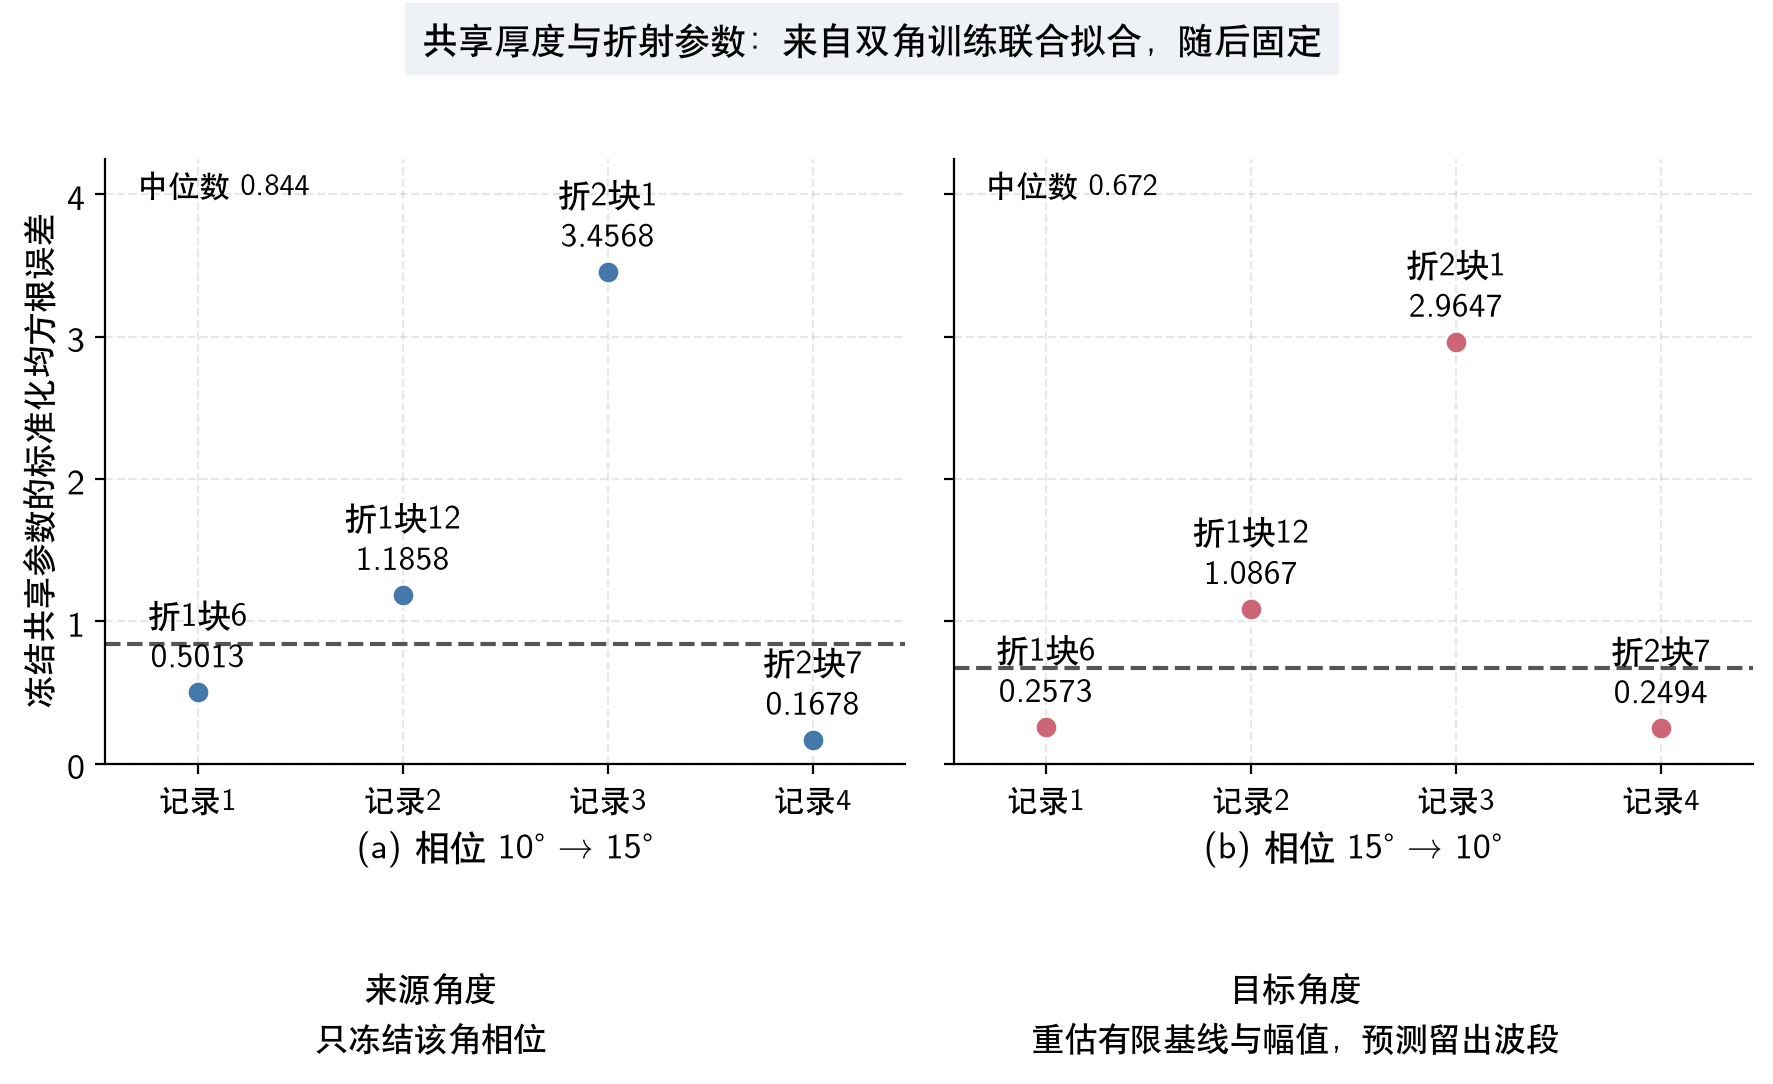
\includegraphics[width=0.8\textwidth]{../求解/问题2/图片/留角度预测核对共享厚度.png}
  \caption{双角参数固定后的跨角响应核对}
  \label{fig:q2-angle}
\end{figure}

完整场的总体误差为$1.0231$，高于两束的$0.9812$；表\ref{tab:supp-q3-blocks}逐块列出同一参数搜索设置下的差值，并与图\ref{fig:17}区分数值核对和图形展示。差值统一取两束误差减完整场误差，正值表示完整场在该块的预测误差较低。
% src:求解/问题3/结果/回炉轮3候选/仲裁闭环/20260910_131501_81623_建模公式/厚度结果.json:分材料验证.硅.逐折汇总.0.平均标准化均方根误差.两束;分材料验证.硅.逐折汇总.0.平均标准化均方根误差.完整往返;分材料验证.硅.逐折汇总.0.平均标准化均方根误差.训练均值;分材料验证.硅.逐折汇总.0.平均标准化均方根误差.二次趋势;分材料验证.硅.逐折汇总.1.平均标准化均方根误差.两束;分材料验证.硅.逐折汇总.1.平均标准化均方根误差.完整往返;分材料验证.硅.逐折汇总.1.平均标准化均方根误差.训练均值;分材料验证.硅.逐折汇总.1.平均标准化均方根误差.二次趋势;分材料验证.碳化硅.逐折汇总.0.平均标准化均方根误差.两束;分材料验证.碳化硅.逐折汇总.0.平均标准化均方根误差.完整往返;分材料验证.碳化硅.逐折汇总.0.平均标准化均方根误差.训练均值;分材料验证.碳化硅.逐折汇总.0.平均标准化均方根误差.二次趋势;分材料验证.碳化硅.逐折汇总.1.平均标准化均方根误差.两束;分材料验证.碳化硅.逐折汇总.1.平均标准化均方根误差.完整往返;分材料验证.碳化硅.逐折汇总.1.平均标准化均方根误差.训练均值;分材料验证.碳化硅.逐折汇总.1.平均标准化均方根误差.二次趋势
% src:交接/实验记录.json:563.尝试;563.现象;563.决定

\begingroup
\small
\setlength{\LTpre}{0pt}
\setlength{\LTpost}{0pt}
\renewcommand{\arraystretch}{1.00}
\begin{longtable}{>{\centering\arraybackslash}p{0.10\textwidth}>{\centering\arraybackslash}p{0.10\textwidth}>{\centering\arraybackslash}p{0.10\textwidth}>{\centering\arraybackslash}p{0.17\textwidth}>{\centering\arraybackslash}p{0.17\textwidth}>{\centering\arraybackslash}p{0.16\textwidth}}
\caption{全部测试块的完整往返与两束误差}\label{tab:supp-q3-blocks}\\
\toprule
附件 & 折号 & 块号 & 两束误差 & 完整往返 & 误差差值 \\
\midrule
\endfirsthead
\caption[]{全部测试块的完整往返与两束误差（续）}\\
\toprule
附件 & 折号 & 块号 & 两束误差 & 完整往返 & 误差差值 \\
\midrule
\endhead
1 & 1 & 6 & 0.1290 & 0.1287 & +0.0003 \\
1 & 1 & 12 & 0.1455 & 0.1460 & -0.0005 \\
1 & 2 & 1 & 2.0936 & 2.1254 & -0.0319 \\
1 & 2 & 7 & 0.1299 & 0.1251 & +0.0048 \\
2 & 1 & 6 & 0.3561 & 0.3504 & +0.0057 \\
2 & 1 & 12 & 0.2853 & 0.2860 & -0.0007 \\
2 & 2 & 1 & 2.4656 & 2.4803 & -0.0147 \\
2 & 2 & 7 & 0.2059 & 0.2013 & +0.0046 \\
3 & 1 & 6 & 0.1401 & 0.0982 & +0.0419 \\
3 & 1 & 12 & 0.2461 & 0.1861 & +0.0600 \\
3 & 2 & 1 & 4.1345 & 4.5085 & -0.3740 \\
3 & 2 & 7 & 0.3344 & 0.3937 & -0.0592 \\
4 & 1 & 6 & 0.3136 & 0.2514 & +0.0621 \\
4 & 1 & 12 & 0.1677 & 0.1115 & +0.0563 \\
4 & 2 & 1 & 4.4083 & 4.7480 & -0.3397 \\
4 & 2 & 7 & 0.1433 & 0.2289 & -0.0856 \\
\bottomrule
\end{longtable}
\endgroup
% src:求解/问题3/结果/回炉轮3候选/仲裁闭环/20260910_131501_81623_建模公式/厚度结果.json:逐块评分.32.标准化均方根误差;逐块评分.36.标准化均方根误差;逐块评分.33.标准化均方根误差;逐块评分.37.标准化均方根误差;逐块评分.48.标准化均方根误差;逐块评分.52.标准化均方根误差;逐块评分.49.标准化均方根误差;逐块评分.53.标准化均方根误差;逐块评分.34.标准化均方根误差;逐块评分.38.标准化均方根误差;逐块评分.35.标准化均方根误差;逐块评分.39.标准化均方根误差;逐块评分.50.标准化均方根误差;逐块评分.54.标准化均方根误差;逐块评分.51.标准化均方根误差;逐块评分.55.标准化均方根误差;逐块评分.0.标准化均方根误差;逐块评分.4.标准化均方根误差;逐块评分.1.标准化均方根误差;逐块评分.5.标准化均方根误差;逐块评分.16.标准化均方根误差;逐块评分.20.标准化均方根误差;逐块评分.17.标准化均方根误差;逐块评分.21.标准化均方根误差;逐块评分.2.标准化均方根误差;逐块评分.6.标准化均方根误差;逐块评分.3.标准化均方根误差;逐块评分.7.标准化均方根误差;逐块评分.18.标准化均方根误差;逐块评分.22.标准化均方根误差;逐块评分.19.标准化均方根误差;逐块评分.23.标准化均方根误差

负差值同时出现在硅与碳化硅，材料、角度和区段都会改变比较方向。上述差值衡量反射率预测，对应表\ref{tab:08}的两材料厚度处理，但不将局部拟合改善直接换算为厚度精度提升。

相位歧义、参考折射率边界和重复相位支持不足，各自对应不同的失败原因。表\ref{tab:supp-failures}连同硅原型的反向收益保存实际记录；其中曾把参考折射率减小$3\%$与触及物理边界后的取值混为一谈，后来将严格扰动和边界情景分开，避免用另一种条件冒充原先的扰动。
% src:交接/实验记录.json:519.尝试;519.现象;519.决定

\begingroup
\small
\begin{longtable}{>{\centering\arraybackslash}p{0.22\textwidth}>{\centering\arraybackslash}p{0.22\textwidth}>{\centering\arraybackslash}p{0.22\textwidth}>{\centering\arraybackslash}p{0.22\textwidth}}
\caption{实际尝试中的歧义与失效记录}\label{tab:supp-failures}\\
\toprule
尝试对象 & 实际现象 & 保留内容 & 解释方式 \\
\midrule
\endfirsthead
\toprule
尝试对象 & 实际现象 & 保留内容 & 解释方式 \\
\midrule
\endhead
合成相位路线 & 近优厚度不唯一 & 保留全部案例 & 候选成对列出 \\
实测折射率扰动 & 请求值越过边界 & 严格与边界分开 & 边界不并入范围 \\
原型周期形状 & 重复相位支持弱 & 保留有限数值 & 形状与机理分开 \\
原型硅往返场 & 分材料收益反向 & 保留硅误差 & 逐块比较方向 \\
\bottomrule
\end{longtable}
\endgroup
% src:求解/问题1/原型结果/路线3.json:辅助诊断.有歧义案例数;合成逐例.0.求解
% src:交接/实验记录.json:58.现象;58.决定;519.现象;519.决定;70.现象;70.决定
% src:求解/问题3/原型结果/锦标赛核验.json:路线三资格诊断;路线核验.0.分材料

这些记录区分了“算出数值”与“识别唯一厚度”两件事，也保留了复杂路线局部变差的证据。路线和失效对象明确后，区间检验进一步核对预测带实际容纳了多少观测。

\subsubsection{区间计数：反射率覆盖与厚度范围分开}

反射率区间检查的是未参与拟合和校准的观测值是否落在预测带内；厚度范围则记录切分与光学条件改变后的取值。两类量分别保存分子、分母和参与比较的对象，以便回查表\ref{tab:09}和表\ref{tab:10}。

碳化硅正式反射率测试共有320点，其中157点落入预测带，经验覆盖率为$49.06\%$；图\ref{fig:q2-coverage}给出局部覆盖形态，表\ref{tab:supp-coverage}补全分角度计数。预测带的半宽取校准块绝对残差的固定经验分位，覆盖率则由测试块另行计算。
% src:求解/问题2/结果/区间覆盖.json:测试点数;测试经验覆盖率;构造方法
% src:求解/问题2/结果/验证.json:分块

问题二实际采用$75\%$校准分位；问题三采用$90\%$校准分位。前者没有设定名义覆盖保证，因此两问覆盖率既要结合各自的预测带构造解释，也要保持反射率与厚度这两类对象的区分。
% src:求解/问题2/结果/区间覆盖.json:校准经验分位点;构造方法
% src:求解/问题3/结果/回炉轮3候选/仲裁闭环/20260910_131501_81623_建模公式/厚度结果.json:预测区间.4.经验覆盖率;预测区间.4.平均区间宽度_比例;预测区间.5.经验覆盖率;预测区间.5.平均区间宽度_比例;预测区间.6.经验覆盖率;预测区间.6.平均区间宽度_比例;预测区间.7.经验覆盖率;预测区间.7.平均区间宽度_比例;预测区间.20.经验覆盖率;预测区间.20.平均区间宽度_比例;预测区间.21.经验覆盖率;预测区间.21.平均区间宽度_比例;预测区间.22.经验覆盖率;预测区间.22.平均区间宽度_比例;预测区间.23.经验覆盖率;预测区间.23.平均区间宽度_比例;预测区间.36.经验覆盖率;预测区间.36.平均区间宽度_比例;预测区间.37.经验覆盖率;预测区间.37.平均区间宽度_比例;预测区间.38.经验覆盖率;预测区间.38.平均区间宽度_比例;预测区间.39.经验覆盖率;预测区间.39.平均区间宽度_比例;预测区间.52.经验覆盖率;预测区间.52.平均区间宽度_比例;预测区间.53.经验覆盖率;预测区间.53.平均区间宽度_比例;预测区间.54.经验覆盖率;预测区间.54.平均区间宽度_比例;预测区间.55.经验覆盖率;预测区间.55.平均区间宽度_比例;预测区间.4.名义覆盖率
% src:求解/问题3/结果/回炉轮3候选/仲裁闭环/20260910_131501_81623_建模公式/厚度结果.json:逐块评分.4.测试点数;逐块评分.5.测试点数;逐块评分.6.测试点数;逐块评分.7.测试点数;逐块评分.20.测试点数;逐块评分.21.测试点数;逐块评分.22.测试点数;逐块评分.23.测试点数;逐块评分.36.测试点数;逐块评分.37.测试点数;逐块评分.38.测试点数;逐块评分.39.测试点数;逐块评分.52.测试点数;逐块评分.53.测试点数;逐块评分.54.测试点数;逐块评分.55.测试点数

完整往返的反射率测试共有640点，其中473点被预测带覆盖，经验覆盖率为$73.91\%$。表\ref{tab:supp-coverage}按材料与角度拆开这个总数，避免把某一材料较宽的预测带当成所有观测都得到同等解释。
% src:求解/问题3/结果/回炉轮3候选/仲裁闭环/20260910_131501_81623_建模公式/厚度结果.json:预测区间.4.经验覆盖率;预测区间.4.平均区间宽度_比例;预测区间.5.经验覆盖率;预测区间.5.平均区间宽度_比例;预测区间.6.经验覆盖率;预测区间.6.平均区间宽度_比例;预测区间.7.经验覆盖率;预测区间.7.平均区间宽度_比例;预测区间.20.经验覆盖率;预测区间.20.平均区间宽度_比例;预测区间.21.经验覆盖率;预测区间.21.平均区间宽度_比例;预测区间.22.经验覆盖率;预测区间.22.平均区间宽度_比例;预测区间.23.经验覆盖率;预测区间.23.平均区间宽度_比例;预测区间.36.经验覆盖率;预测区间.36.平均区间宽度_比例;预测区间.37.经验覆盖率;预测区间.37.平均区间宽度_比例;预测区间.38.经验覆盖率;预测区间.38.平均区间宽度_比例;预测区间.39.经验覆盖率;预测区间.39.平均区间宽度_比例;预测区间.52.经验覆盖率;预测区间.52.平均区间宽度_比例;预测区间.53.经验覆盖率;预测区间.53.平均区间宽度_比例;预测区间.54.经验覆盖率;预测区间.54.平均区间宽度_比例;预测区间.55.经验覆盖率;预测区间.55.平均区间宽度_比例;预测区间.4.名义覆盖率
% src:求解/问题3/结果/回炉轮3候选/仲裁闭环/20260910_131501_81623_建模公式/厚度结果.json:逐块评分.4.测试点数;逐块评分.5.测试点数;逐块评分.6.测试点数;逐块评分.7.测试点数;逐块评分.20.测试点数;逐块评分.21.测试点数;逐块评分.22.测试点数;逐块评分.23.测试点数;逐块评分.36.测试点数;逐块评分.37.测试点数;逐块评分.38.测试点数;逐块评分.39.测试点数;逐块评分.52.测试点数;逐块评分.53.测试点数;逐块评分.54.测试点数;逐块评分.55.测试点数

\begingroup
\small
\begin{longtable}{>{\centering\arraybackslash}p{0.12\textwidth}>{\centering\arraybackslash}p{0.14\textwidth}>{\centering\arraybackslash}p{0.12\textwidth}>{\centering\arraybackslash}p{0.14\textwidth}>{\centering\arraybackslash}p{0.14\textwidth}>{\centering\arraybackslash}p{0.14\textwidth}}
\caption{反射率测试覆盖的分材料分角计数}\label{tab:supp-coverage}\\
\toprule
问题 & 材料 & 角度 & 覆盖点 & 测试点 & 覆盖（\%） \\
\midrule
\endfirsthead
\toprule
问题 & 材料 & 角度 & 覆盖点 & 测试点 & 覆盖（\%） \\
\midrule
\endhead
问题三 & 硅 & $10^\circ$ & 119 & 160 & 74.38 \\
问题三 & 硅 & $15^\circ$ & 123 & 160 & 76.88 \\
问题三 & 碳化硅 & $10^\circ$ & 132 & 160 & 82.50 \\
问题三 & 碳化硅 & $15^\circ$ & 99 & 160 & 61.88 \\
问题二 & 碳化硅 & $10^\circ$ & 84 & 160 & 52.50 \\
问题二 & 碳化硅 & $15^\circ$ & 73 & 160 & 45.63 \\
问题二 & 合计 & --- & 157 & 320 & 49.06 \\
问题三 & 合计 & --- & 473 & 640 & 73.91 \\
\bottomrule
\end{longtable}
\endgroup
% src:求解/问题2/结果/验证.json:分块
% src:求解/问题2/结果/区间覆盖.json:测试经验覆盖率;测试点数
% src:求解/问题3/结果/回炉轮3候选/仲裁闭环/20260910_131501_81623_建模公式/厚度结果.json:逐块评分.32.标准化均方根误差;逐块评分.36.标准化均方根误差;逐块评分.33.标准化均方根误差;逐块评分.37.标准化均方根误差;逐块评分.48.标准化均方根误差;逐块评分.52.标准化均方根误差;逐块评分.49.标准化均方根误差;逐块评分.53.标准化均方根误差;逐块评分.34.标准化均方根误差;逐块评分.38.标准化均方根误差;逐块评分.35.标准化均方根误差;逐块评分.39.标准化均方根误差;逐块评分.50.标准化均方根误差;逐块评分.54.标准化均方根误差;逐块评分.51.标准化均方根误差;逐块评分.55.标准化均方根误差;逐块评分.0.标准化均方根误差;逐块评分.4.标准化均方根误差;逐块评分.1.标准化均方根误差;逐块评分.5.标准化均方根误差;逐块评分.16.标准化均方根误差;逐块评分.20.标准化均方根误差;逐块评分.17.标准化均方根误差;逐块评分.21.标准化均方根误差;逐块评分.2.标准化均方根误差;逐块评分.6.标准化均方根误差;逐块评分.3.标准化均方根误差;逐块评分.7.标准化均方根误差;逐块评分.18.标准化均方根误差;逐块评分.22.标准化均方根误差;逐块评分.19.标准化均方根误差;逐块评分.23.标准化均方根误差
% src:求解/问题3/结果/回炉轮3候选/仲裁闭环/20260910_131501_81623_建模公式/厚度结果.json:预测区间.4.经验覆盖率;预测区间.4.平均区间宽度_比例;预测区间.5.经验覆盖率;预测区间.5.平均区间宽度_比例;预测区间.6.经验覆盖率;预测区间.6.平均区间宽度_比例;预测区间.7.经验覆盖率;预测区间.7.平均区间宽度_比例;预测区间.20.经验覆盖率;预测区间.20.平均区间宽度_比例;预测区间.21.经验覆盖率;预测区间.21.平均区间宽度_比例;预测区间.22.经验覆盖率;预测区间.22.平均区间宽度_比例;预测区间.23.经验覆盖率;预测区间.23.平均区间宽度_比例;预测区间.36.经验覆盖率;预测区间.36.平均区间宽度_比例;预测区间.37.经验覆盖率;预测区间.37.平均区间宽度_比例;预测区间.38.经验覆盖率;预测区间.38.平均区间宽度_比例;预测区间.39.经验覆盖率;预测区间.39.平均区间宽度_比例;预测区间.52.经验覆盖率;预测区间.52.平均区间宽度_比例;预测区间.53.经验覆盖率;预测区间.53.平均区间宽度_比例;预测区间.54.经验覆盖率;预测区间.54.平均区间宽度_比例;预测区间.55.经验覆盖率;预测区间.55.平均区间宽度_比例;预测区间.4.名义覆盖率
% src:求解/问题3/结果/回炉轮3候选/仲裁闭环/20260910_131501_81623_建模公式/厚度结果.json:逐块评分.4.测试点数;逐块评分.5.测试点数;逐块评分.6.测试点数;逐块评分.7.测试点数;逐块评分.20.测试点数;逐块评分.21.测试点数;逐块评分.22.测试点数;逐块评分.23.测试点数;逐块评分.36.测试点数;逐块评分.37.测试点数;逐块评分.38.测试点数;逐块评分.39.测试点数;逐块评分.52.测试点数;逐块评分.53.测试点数;逐块评分.54.测试点数;逐块评分.55.测试点数

这些分母统计的是连续测试块内的反射率观测，而非独立晶圆数。厚度随条件改变的范围不参与覆盖计数；它们在表\ref{tab:supp-range}中按形成方式另列，其中碳化硅的范围为$0.6367$--$18.1064\ \mu\mathrm m$，来自切分、光学剖面和合法参数情景的并集。
% src:求解/问题2/结果/厚度结果.json:条件区间_微米;条件区间组成;条件区间构造

\begingroup
\small
\begin{longtable}{>{\centering\arraybackslash}p{0.24\textwidth}>{\centering\arraybackslash}p{0.20\textwidth}>{\centering\arraybackslash}p{0.20\textwidth}>{\centering\arraybackslash}p{0.24\textwidth}}
\caption{厚度范围与形成对象分别对应}\label{tab:supp-range}\\
\toprule
对象 & 下限（$\mu\mathrm m$） & 上限（$\mu\mathrm m$） & 范围形成方式 \\
\midrule
\endfirsthead
\toprule
对象 & 下限（$\mu\mathrm m$） & 上限（$\mu\mathrm m$） & 范围形成方式 \\
\midrule
\endhead
问题一合成扰动 & 6.6622 & 10.0142 & 同一锚例重估 \\
问题二碳化硅 & 0.6367 & 18.1064 & 切分与情景并集 \\
问题三硅两折 & 1.7322 & 16.0424 & 连续留段折间范围 \\
问题三硅包络 & 1.7246 & 18.1553 & 非概率情景联合包络 \\
问题三碳化硅 & 0.6367 & 18.1064 & 沿用问题二基准 \\
\bottomrule
\end{longtable}
\endgroup
% src:求解/问题1/结果/灵敏度.json:条件压力范围_微米
% src:求解/问题2/结果/厚度结果.json:条件区间_微米;条件区间组成
% src:求解/问题3/结果/回炉轮3候选/仲裁闭环/20260910_131501_81623_建模公式/厚度结果.json:核心指标.硅折1完整往返条件厚度_um;核心指标.硅折2完整往返条件厚度_um;核心指标.碳化硅正式条件范围下限_um;核心指标.碳化硅正式条件范围上限_um

折间范围来自重估条件的变化，主窗口全量拟合则使用另一组观测对象：硅每角保留5392个原始点，给出的厚度为$2.1651\ \mu\mathrm m$。同段两束值为$2.3193\ \mu\mathrm m$，完整往返减两束为$-0.1542\ \mu\mathrm m$。
% src:求解/问题3/结果/回炉轮3候选/仲裁闭环/20260910_131501_81623_建模公式/厚度结果.json:案例.0.最优.厚度_um;案例.1.最优.厚度_um;案例.6.最优.厚度_um;案例.7.最优.厚度_um

硅两折相差$14.3102\ \mu\mathrm m$，完整包络为$1.7246$--$18.1553\ \mu\mathrm m$。全量值、两折跨度与包含近优候选和扰动的情景包络各有不同统计对象。
% src:求解/问题3/结果/回炉轮3候选/仲裁闭环/20260910_131501_81623_建模公式/厚度结果.json:核心指标.硅全量完整往返厚度_um;核心指标.硅折1完整往返条件厚度_um;核心指标.硅折2完整往返条件厚度_um;核心指标.硅已计算条件包络下限_um;核心指标.硅已计算条件包络上限_um;核心指标.碳化硅正式基准厚度_um;核心指标.碳化硅正式条件范围下限_um;核心指标.碳化硅正式条件范围上限_um
% src:求解/问题3/结果/解读核验_回炉3_仲裁后.json:防泄漏.全量每角点数
% src:求解/问题3/结果/回炉轮3候选/仲裁闭环/20260910_131501_81623_建模公式/厚度结果.json:核心指标.硅全量完整往返厚度_um

历史窗口扰动保留原训练块成员并取窗口交集；表\ref{tab:supp-window-sensitivity}列出当时参与重估的训练点数与厚度，与图\ref{fig:19}的原参数扰动对象对应。点数是各折训练源行的数量，不再把整个切窗样本数写成实际训练点数；该历史表中的范围不代表本次条件包络端点。
% src:求解/问题3/结果/灵敏度.json:灵敏度_参数扰动
% src:交接/实验记录.json:564.尝试;564.现象;564.决定

\begin{figure}[!htb]
  \centering
  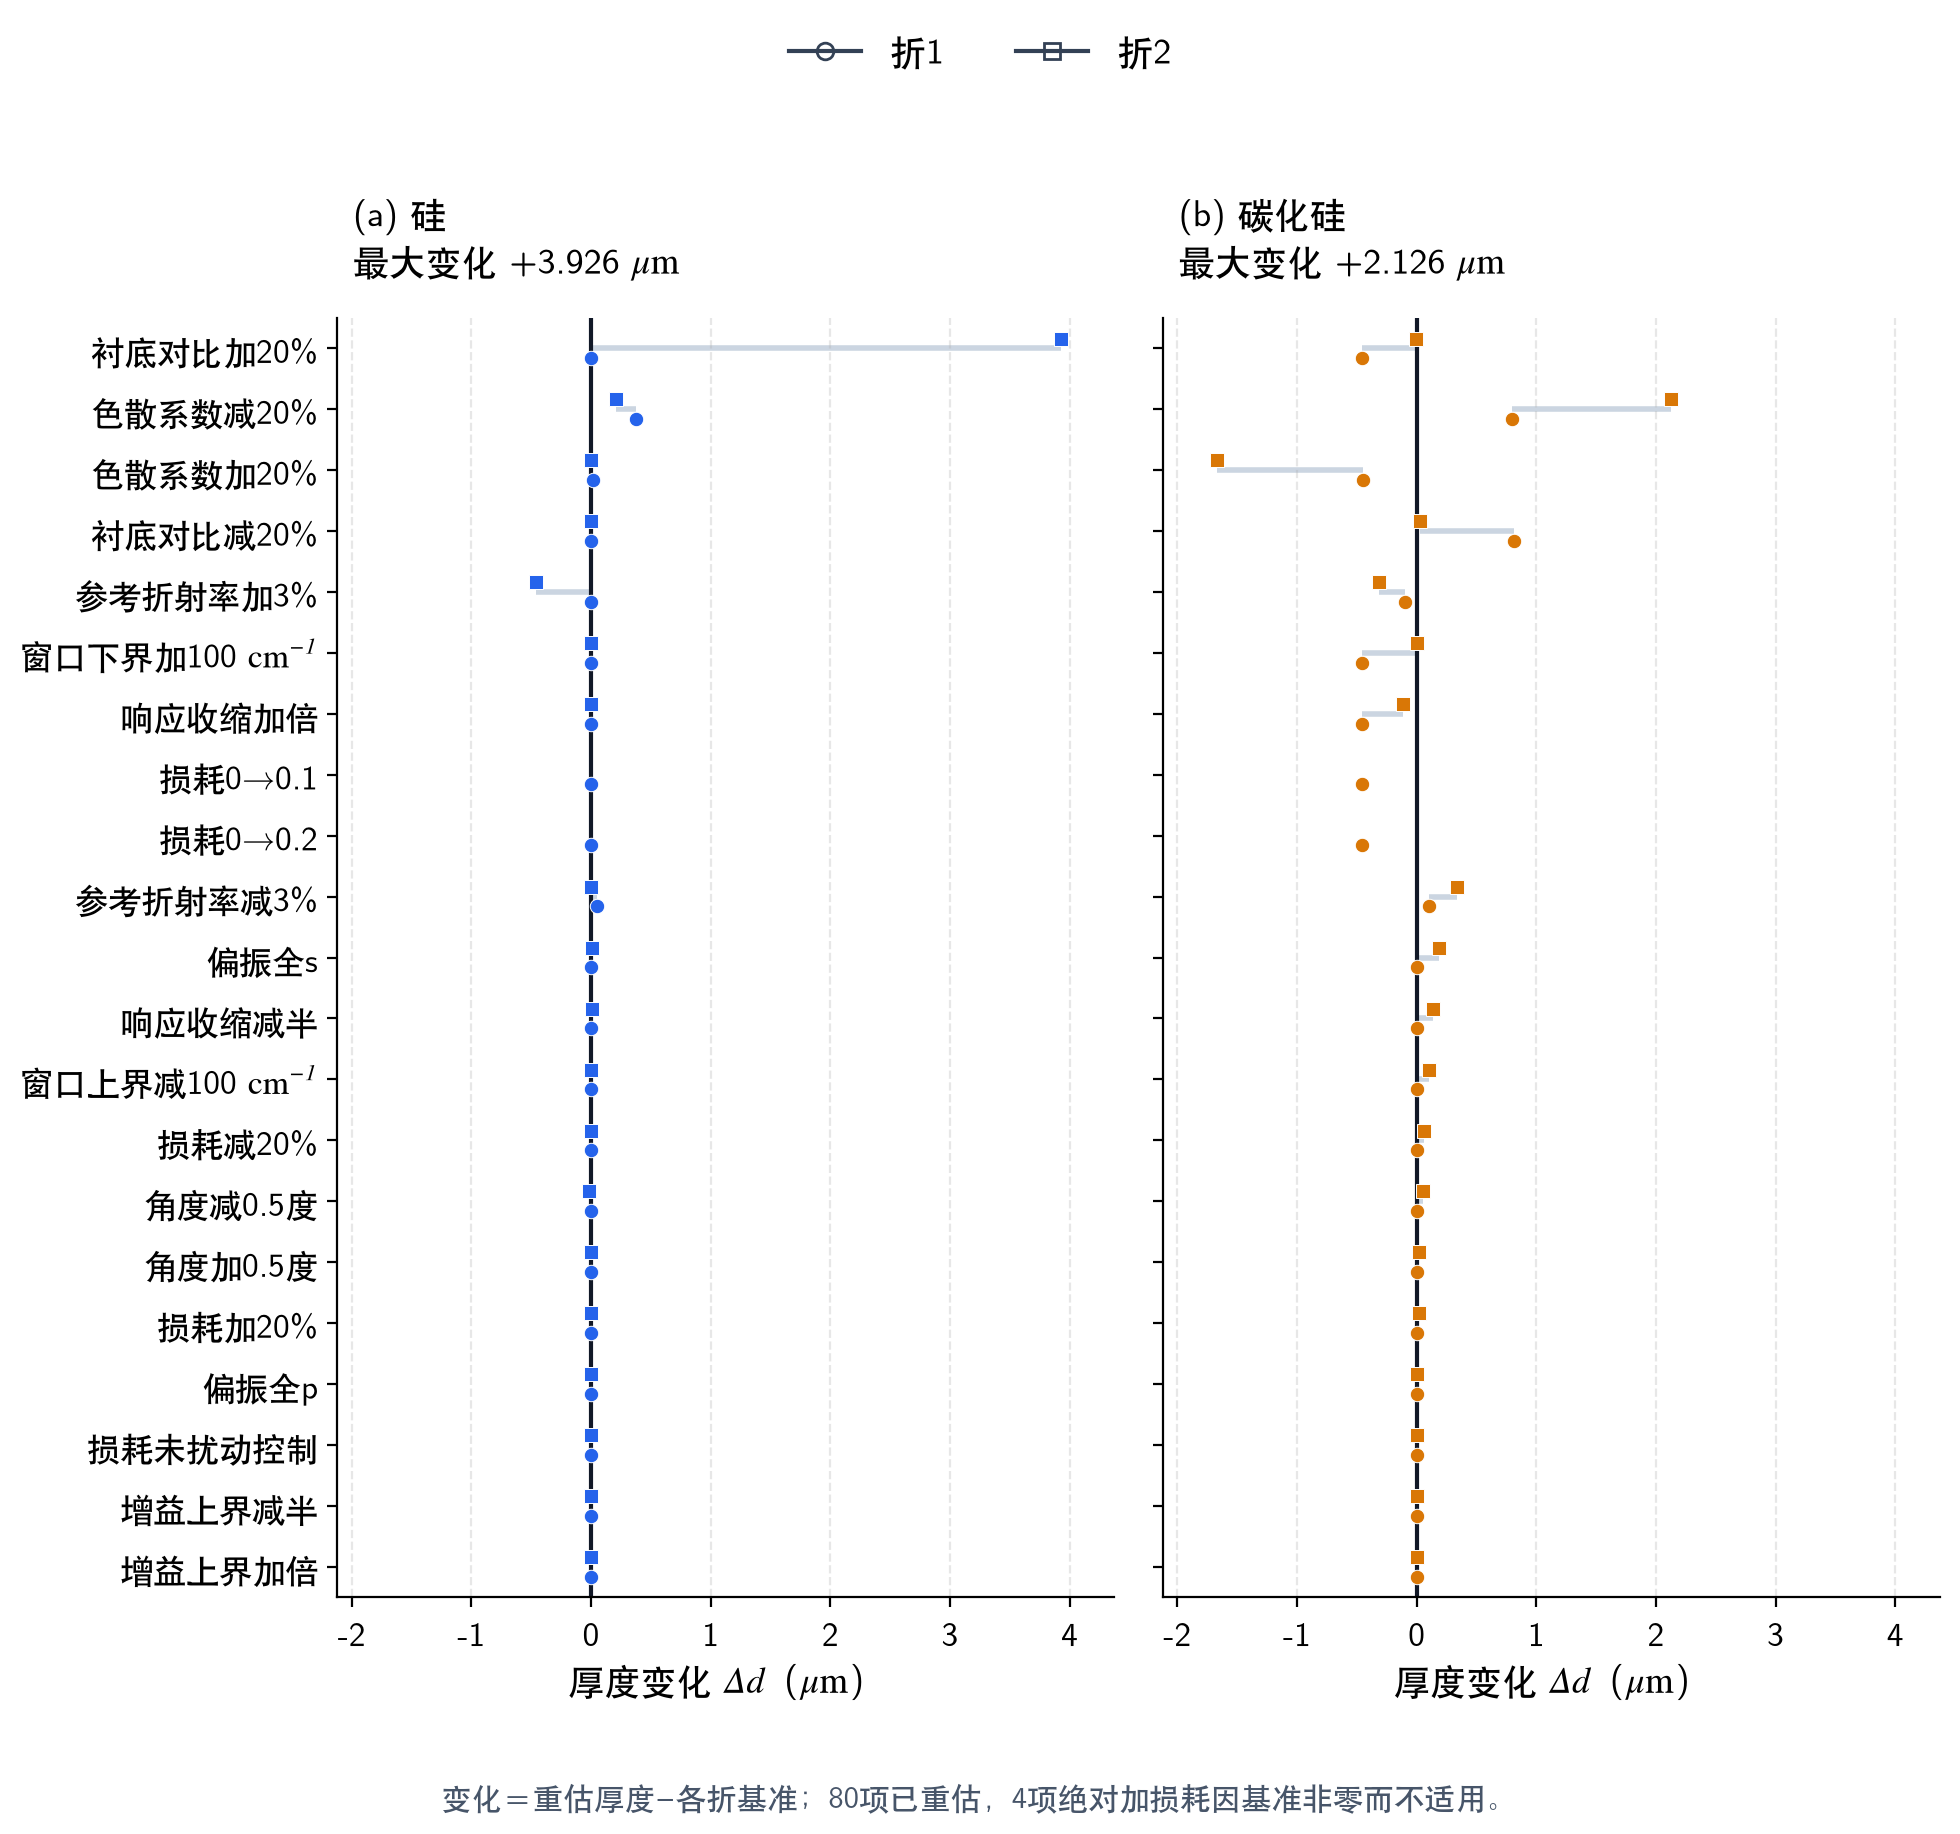
\includegraphics[width=0.8\textwidth]{../求解/问题3/图片/厚度扰动区分谱形与测厚影响.png}
  \caption{两材料厚度随参数扰动发生偏移}
  \label{fig:19}
\end{figure}

\begingroup
\small
\begin{longtable}{>{\centering\arraybackslash}p{0.14\textwidth}>{\centering\arraybackslash}p{0.08\textwidth}>{\centering\arraybackslash}p{0.26\textwidth}>{\centering\arraybackslash}p{0.12\textwidth}>{\centering\arraybackslash}p{0.24\textwidth}}
\caption{历史窗口扰动的点数与重估厚度}\label{tab:supp-window-sensitivity}\\
\toprule
材料 & 折号 & 窗口（$\mathrm{cm}^{-1}$） & 训练点数 & 厚度（$\mu\mathrm m$） \\
\midrule
\endfirsthead
\toprule
材料 & 折号 & 窗口（$\mathrm{cm}^{-1}$） & 训练点数 & 厚度（$\mu\mathrm m$） \\
\midrule
\endhead
硅 & 1 & 1300--3800 & 273 & 1.7345 \\
硅 & 1 & 1200--3700 & 292 & 1.7321 \\
硅 & 2 & 1300--3800 & 292 & 16.0426 \\
硅 & 2 & 1200--3700 & 273 & 16.0424 \\
碳化硅 & 1 & 1300--3800 & 273 & 2.7611 \\
碳化硅 & 1 & 1200--3700 & 292 & 3.2168 \\
碳化硅 & 2 & 1300--3800 & 292 & 10.6616 \\
碳化硅 & 2 & 1200--3700 & 273 & 10.7635 \\
\bottomrule
\end{longtable}
\endgroup
% src:求解/问题3/结果/灵敏度.json:灵敏度_参数扰动

下界内移时按原始波数筛选训练成员，未在端点外插观测。各折训练源行分别保留，窗口变化和区段切分据此具有明确的样本对象。
% src:求解/问题3/结果/灵敏度.json:灵敏度_参数扰动

上界内移采用同一交集规则；重估厚度对照未扰动的同折解，而不与另一折或全量拟合混合。
% src:求解/问题3/结果/灵敏度.json:灵敏度_参数扰动

历史参数与窗口对照共列84项情景，其中80项完成重估，4项因适用条件不满足而单列。表\ref{tab:supp-all-sensitivity}保留原材料和折次的厚度变化；这些差值相对于当时的同折完整往返解，区别于本次同起点控制差，碳化硅的往返对照与问题二采用值也分别承担不同任务。
% src:求解/问题3/结果/灵敏度.json:灵敏度_参数扰动

\begingroup
\small
\setlength{\LTpre}{0pt}
\setlength{\LTpost}{0pt}
\renewcommand{\arraystretch}{1.00}
\begin{longtable}{>{\centering\arraybackslash}p{0.28\textwidth}>{\centering\arraybackslash}p{0.14\textwidth}>{\centering\arraybackslash}p{0.14\textwidth}>{\centering\arraybackslash}p{0.14\textwidth}>{\centering\arraybackslash}p{0.14\textwidth}}
\caption{历史扰动的厚度变化量（微米）}\label{tab:supp-all-sensitivity}\\
\toprule
扰动情景 & 硅首折 & 硅次折 & 碳化硅首折 & 碳化硅次折 \\
\midrule
\endfirsthead
\caption[]{历史扰动的厚度变化量（微米，续）}\\
\toprule
扰动情景 & 硅首折 & 硅次折 & 碳化硅首折 & 碳化硅次折 \\
\midrule
\endhead
有效损耗未扰动控制 & +0.0000 & +0.0002 & +0.0000 & +0.0000 \\
有效损耗减20\% & +0.0000 & +0.0002 & +0.0000 & +0.0648 \\
有效损耗加20\% & +0.0000 & +0.0002 & +0.0000 & +0.0164 \\
有效损耗绝对增加$0\to$0.1 & +0.0003 & 不适用 & -0.4553 & 不适用 \\
有效损耗绝对增加$0\to$0.2 & +0.0006 & 不适用 & -0.4552 & 不适用 \\
衬底对比减20\% & +0.0006 & +0.0026 & +0.8142 & +0.0303 \\
衬底对比加20\% & +0.0000 & +3.9259 & -0.4552 & -0.0037 \\
参考折射率减3\% & +0.0535 & +0.0002 & +0.0997 & +0.3370 \\
参考折射率加3\% & +0.0000 & -0.4571 & -0.0939 & -0.3168 \\
色散系数减20\% & +0.3767 & +0.2068 & +0.7962 & +2.1261 \\
色散系数加20\% & +0.0152 & +0.0000 & -0.4521 & -1.6720 \\
偏振全$s$ & +0.0000 & +0.0063 & +0.0000 & +0.1841 \\
偏振全$p$ & +0.0000 & -0.0001 & -0.0002 & +0.0000 \\
入射角同时减0.5度 & -0.0001 & -0.0159 & -0.0002 & +0.0509 \\
入射角同时加0.5度 & +0.0001 & +0.0000 & +0.0000 & +0.0208 \\
窗口下界加100 & +0.0024 & +0.0002 & -0.4557 & +0.0000 \\
窗口上界减100 & +0.0000 & +0.0000 & +0.0000 & +0.1019 \\
响应收缩减半 & +0.0001 & +0.0064 & +0.0002 & +0.1342 \\
响应收缩加倍 & -0.0001 & +0.0002 & -0.4555 & -0.1147 \\
标准化增益上界减半 & +0.0000 & +0.0002 & +0.0000 & +0.0000 \\
标准化增益上界加倍 & +0.0000 & +0.0002 & +0.0000 & +0.0000 \\
\bottomrule
\end{longtable}
\endgroup
% src:求解/问题3/结果/灵敏度.json:灵敏度_参数扰动

扰动结果同时保留变大、变小与显示精度下不变的取值；它们记录特定光学条件附近的重估响应，而不是给观测增加独立重复次数。源附件、比较路线、失败原因、覆盖计数与有效点数至此逐一对应，正文的各项结论均可回到相同对象核查。

\begingroup
\setlength{\intextsep}{4pt plus 1pt minus 1pt}
\setlength{\textfloatsep}{4pt plus 1pt minus 1pt}
\subsubsection{补充图证：场展开与色散响应}

场展开的两种表达在图\ref{fig:field-expansion}中逐点对照，比较对象为合场强度与交叉项展开。

\begin{figure}[!htb]
  \centering
  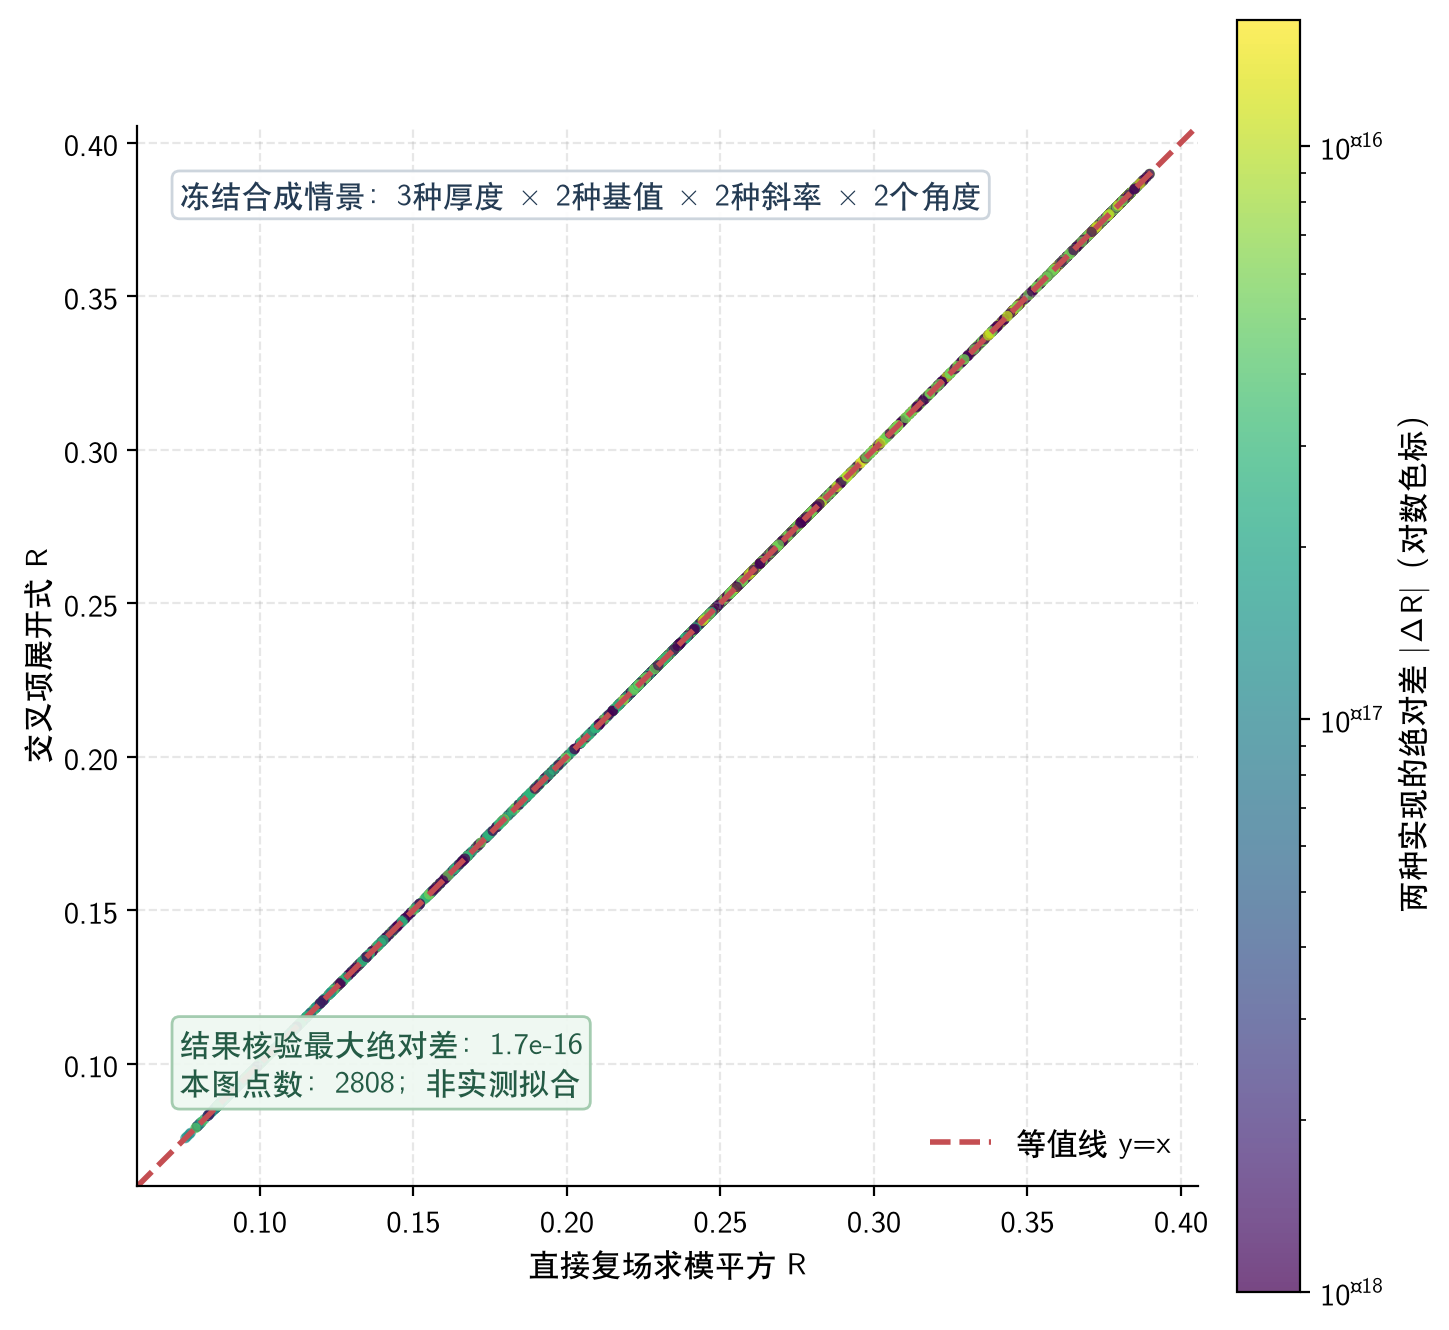
\includegraphics[width=0.8\textwidth]{../求解/问题1/图片/场求和与展开强度相符.png}
  \caption{两种强度展开实现的逐点一致性}
  \label{fig:field-expansion}
\end{figure}

图\ref{fig:dispersion-spacing}呈现折射变化对局部峰距的影响，与常折射率近似比较。

\begin{figure}[!htb]
  \centering
  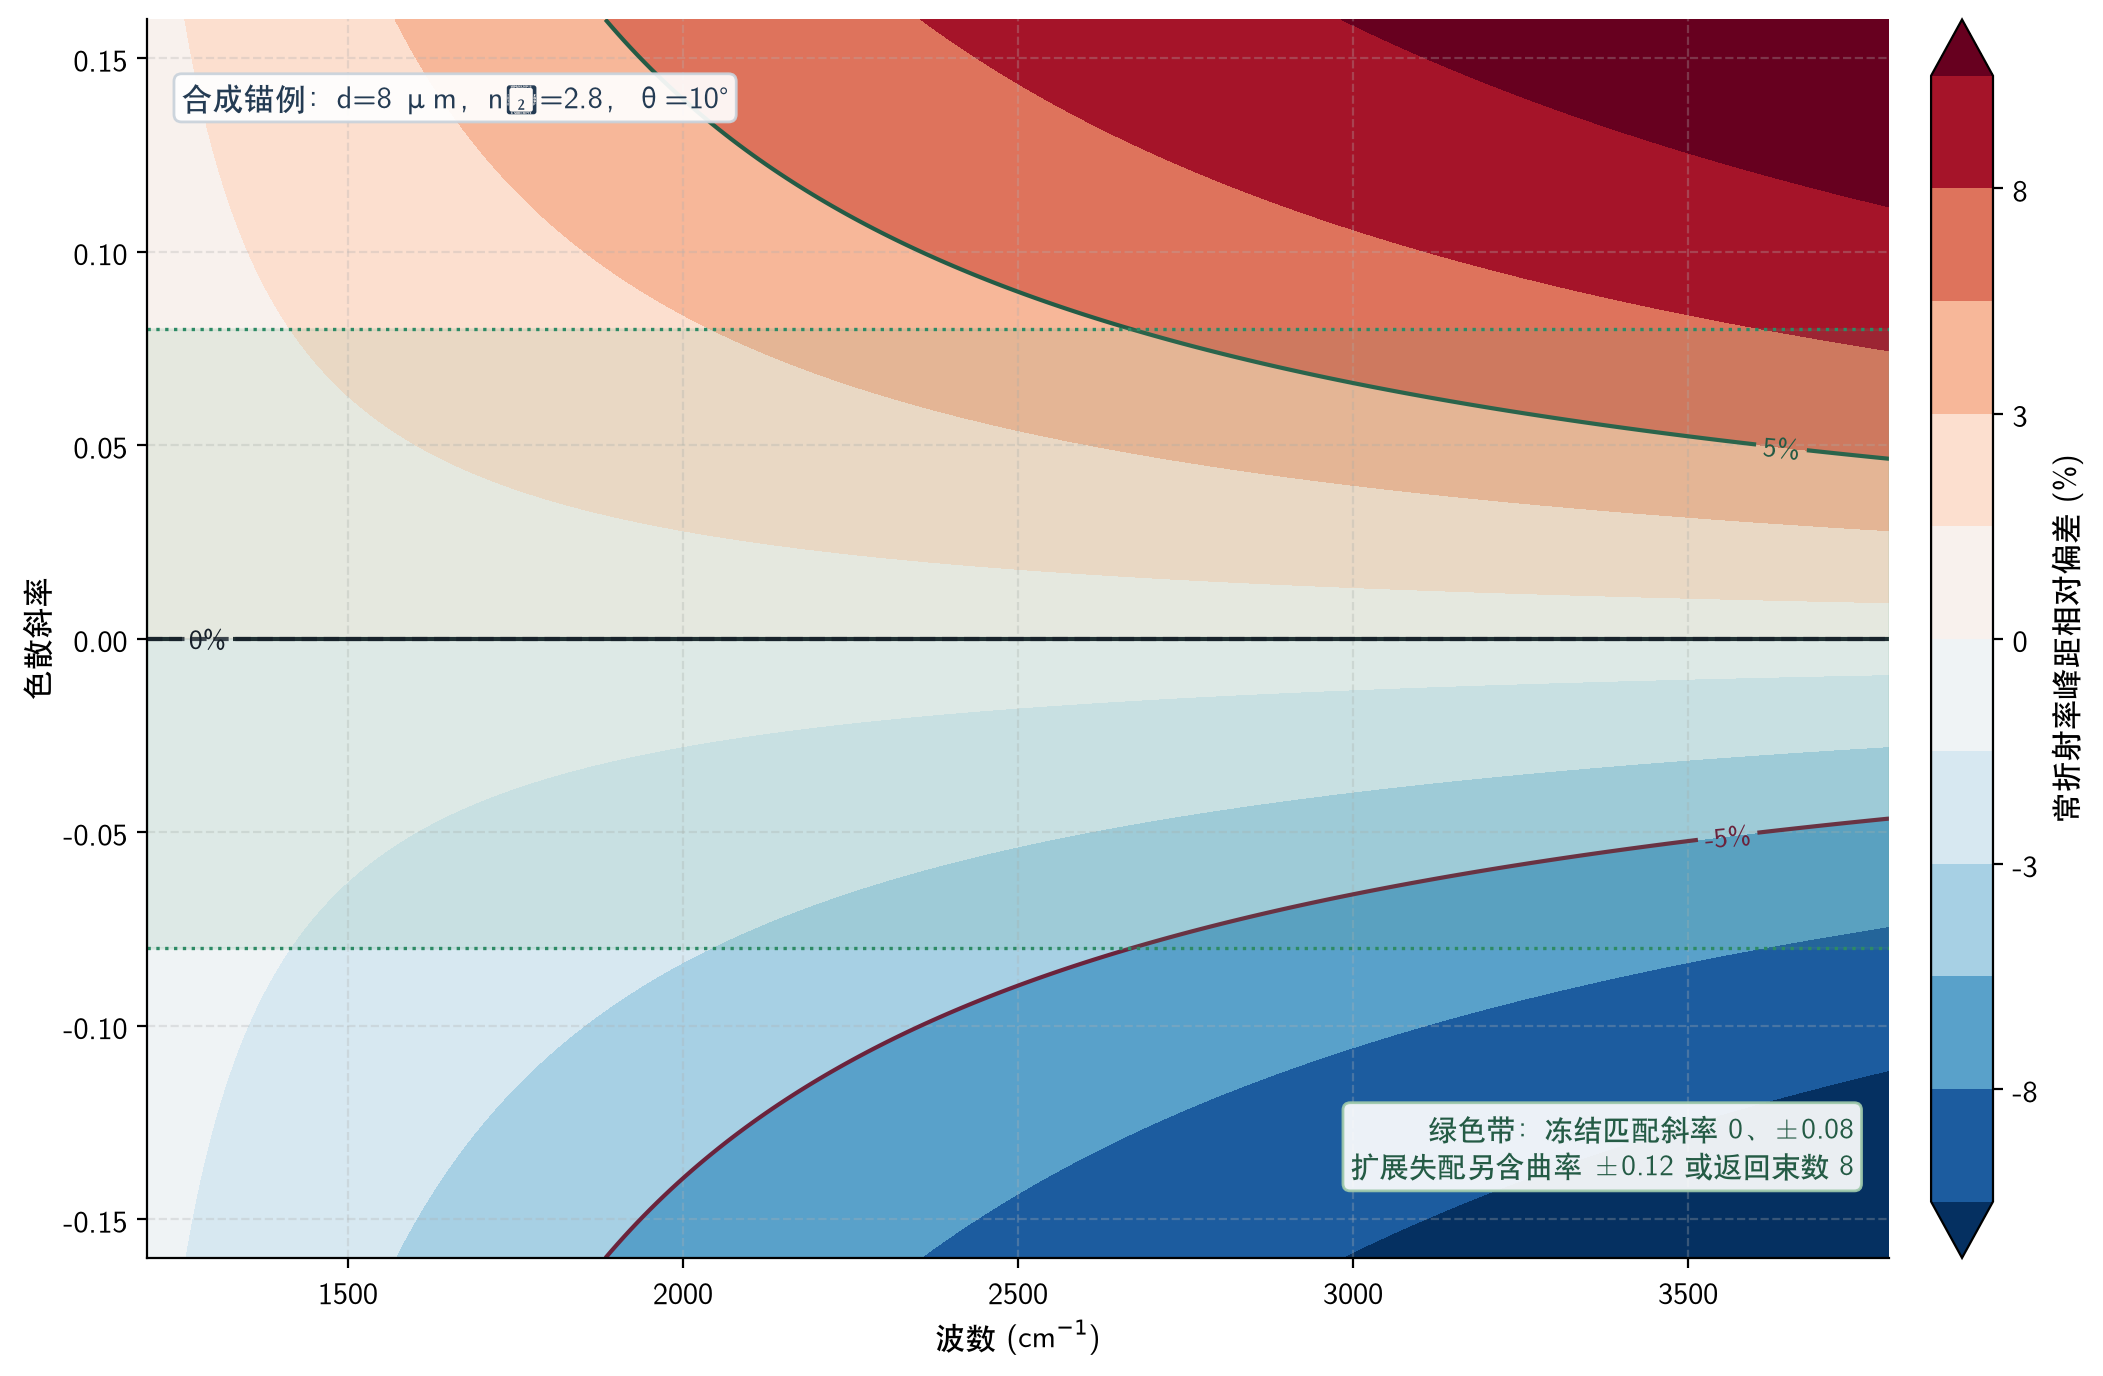
\includegraphics[width=0.8\textwidth]{../求解/问题1/图片/色散斜率改变局部峰距.png}
  \caption{色散斜率对局部峰距偏差的影响}
  \label{fig:dispersion-spacing}
\end{figure}
\endgroup
